\section{数学环境}

我们可以使用标准的 LaTeX 数学环境。

行内公式:$E = mc^2$。

行间公式:
\[
    \int_{-\infty}^{\infty} e^{-x^2} \, dx = \sqrt{\pi}
\]

\begin{thmbox}[微积分基本定理]{ftc}
    设 $f$ 是定义在闭区间 $[a, b]$ 上的连续实值函数。设 $F$ 是定义在 $[a, b]$ 上的函数,对于所有 $x \in [a, b]$,有
    \[
        F(x) = \int_a^x f(t) \, dt
    \]
    则 $F$ 在 $[a, b]$ 上一致连续,在开区间 $(a, b)$ 上可导,并且对于所有 $x \in (a, b)$,有
    \[
        F'(x) = f(x)
    \]
\end{thmbox}

\begin{lembox}[夹逼定理]{squeeze}
    如果 $g(x) \leq f(x) \leq h(x)$ 且 $\lim_{x \to a} g(x) = \lim_{x \to a} h(x) = L$,那么 $\lim_{x \to a} f(x) = L$。
\end{lembox}

\section{文本块}

\begin{dfnbox}[极限的定义]{limit-def}
    设 $f$ 是定义在包含 $c$ 的开区间(可能除去 $c$ 点)上的函数,且 $L$ 是一个实数。语句
    \[
        \lim_{x \to c} f(x) = L
    \]
    意味着对于任意 $\epsilon > 0$,存在一个 $\delta > 0$,使得如果 $0 < |x - c| < \delta$,则 $|f(x) - L| < \epsilon$。
\end{dfnbox}

\begin{exbox}[计算示例]{ex1}
    计算 $x \to 2$ 时 $f(x) = x^2$ 的极限。
    
    \textit{解:} 因为 $f(x)$ 是连续的,我们直接代入数值:
    \[
        \lim_{x \to 2} x^2 = 2^2 = 4
    \]
\end{exbox}

\begin{tecbox}[分部积分法]{int-parts}
    分部积分公式为:
    \[
        \int u \, dv = uv - \int v \, du
    \]
    当被积函数是两个函数的乘积时非常有用。
\end{tecbox}

\begin{notebox}
    这是一个简单的提示框。用于强调重要信息或警告。
\end{notebox}

\begin{genbox}{通用信息}
    这是一个通用盒子。可用于任何需要与正文区分的内容。
\end{genbox}

\section{代码块}

由于 \texttt{code} 选项当前已禁用(需要 Python 和 Pygments),这里展示一个使用盒子包裹 \texttt{verbatim} 的模拟代码块。

\begin{tcolorbox}[colback=gray!10, colframe=gray!50, title=Python 示例]
\begin{verbatim}
def hello_world():
    print("Hello, World!")
    return True

if __name__ == "__main__":
    hello_world()
\end{verbatim}
\end{tcolorbox}

如果你在 \texttt{documentclass} 中启用了 \texttt{code} 选项,你可以使用 \texttt{amzcode} 环境进行语法高亮:

\begin{verbatim}
\begin{amzcode}{python}
def hello_world():
    print("Hello, World!")
\end{amzcode}
\end{verbatim}

\section{图片与子图}

\begin{figure}[htbp]
    \centering
    \begin{tikzpicture}
        \draw[fill=amzchaptercolor!20, draw=amzchaptercolor, thick] (0,0) circle (1.5cm);
        \node at (0,0) {\sffamily\bfseries 圆};
    \end{tikzpicture}
    \caption{使用 TikZ 绘制的示例图片}
    \label{fig:circle}
\end{figure}

我们也可以并排排列图片。

\begin{figure}[htbp]
    \centering
    \begin{subfigure}[b]{0.45\textwidth}
        \centering
        \begin{tikzpicture}
            \draw[fill=amzthmboxcolor!20, draw=amzthmboxcolor, thick] (0,0) rectangle (3,2);
            \node at (1.5,1) {A};
        \end{tikzpicture}
        \caption{子图 A}
        \label{fig:subA}
    \end{subfigure}
    \hfill
    \begin{subfigure}[b]{0.45\textwidth}
        \centering
        \begin{tikzpicture}
            \draw[fill=amzexboxcolor!20, draw=amzexboxcolor, thick] (0,0) -- (1.5,2) -- (3,0) -- cycle;
            \node at (1.5,0.7) {B};
        \end{tikzpicture}
        \caption{子图 B}
        \label{fig:subB}
    \end{subfigure}
    \caption{并排的两个子图}
    \label{fig:subfigures}
\end{figure}

\section{表格}

这是一个使用 \texttt{booktabs} 的专业三线表示例。

\begin{table}[htbp]
    \centering
    \caption{模型对比}
    \label{tab:comparison}
    \begin{tabular}{lcr}
        \toprule
        \textbf{模型} & \textbf{准确率} & \textbf{时间 (ms)} \\
        \midrule
        基准模型 & 85.4\% & 12.5 \\
        模型 A  & 88.2\% & 15.3 \\
        模型 B  & 91.7\% & 22.1 \\
        \bottomrule
    \end{tabular}
\end{table}

\section{高级 TikZ 示例}

\subsection{分形 (L-System)}

这是一个使用 Lindenmayer 系统生成的植物分形。

\begin{figure}[htbp]
    \centering
    \begin{tikzpicture}
        \draw [green!50!black, rotate=90]
        [l-system={rule set={F -> F[-F]F[+F][F]}, axiom=F, order=4, step=2pt, angle=25}]
        l-system; 
    \end{tikzpicture}
    \caption{植物分形}
    \label{fig:fractal}
\end{figure}

\subsection{复变函数可视化}

这是一个使用 \texttt{pgfplots} 绘制的函数 $z = x e^{-x^2-y^2}$ 的 3D 图。

\begin{figure}[htbp]
    \centering
    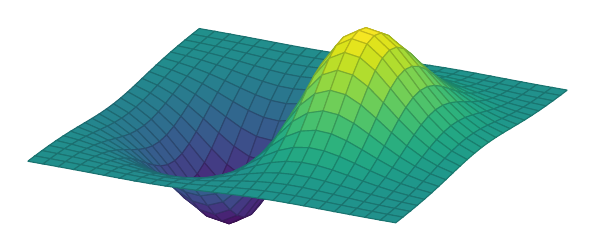
\begin{tikzpicture}
        \begin{axis}[
            colormap/viridis,
            hide axis,
        ]
        \addplot3[
            surf,
            domain=-2:2,
            domain y=-2:2,
        ]
        {exp(-x^2-y^2)*x};
        \end{axis}
    \end{tikzpicture}
    \caption{3D 曲面图}
    \label{fig:surface}
\end{figure}

\subsection{韦恩图}

表示三个集合 $A$、$B$ 和 $C$ 交集的韦恩图。

\begin{figure}[htbp]
    \centering
    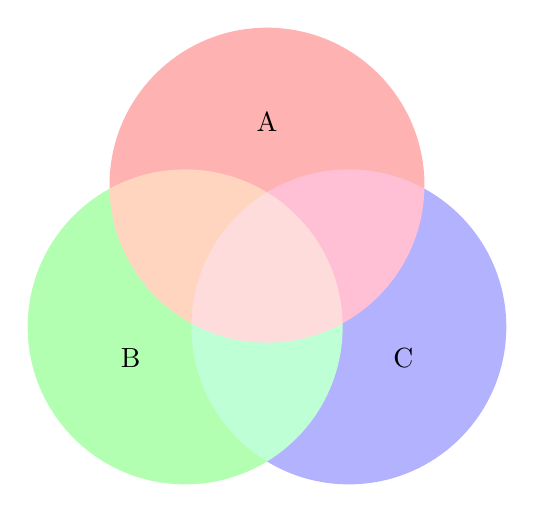
\begin{tikzpicture}
        \begin{scope}[blend group = soft light]
            \fill[red!30!white]   ( 90:1.2) circle (2);
            \fill[green!30!white] (210:1.2) circle (2);
            \fill[blue!30!white]  (330:1.2) circle (2);
        \end{scope}
        \node at ( 90:2)    {A};
        \node at ( 210:2)   {B};
        \node at ( 330:2)   {C};
    \end{tikzpicture}
    \caption{三个集合的韦恩图}
    \label{fig:venn}
\end{figure}

\section{对照块}

我们可以使用 \texttt{comparison} 环境并排对比两个概念。

\begin{comparison}
    \textbf{牛顿力学}
    
    \begin{itemize}
        \item 适用于宏观物体。
        \item 速度远小于光速。
        \item 空间和时间是绝对的。
        \item $F = ma$
    \end{itemize}
    
    \tcblower
    
    \textbf{相对论力学}
    
    \begin{itemize}
        \item 适用于所有速度。
        \item 接近光速时必须使用。
        \item 空间和时间是相对的。
        \item $E = mc^2$
    \end{itemize}
\end{comparison}

\section{Mac 风格代码块}

我们提供两种风格的代码块:浅色和深色。

\subsection{浅色模式}

\begin{maccode}[Python]{hello.py}
def factorial(n):
    """Calculates the factorial of n."""
    if n == 0:
        return 1
    else:
        return n * factorial(n-1)

print(factorial(5))
\end{maccode}

\subsection{深色模式}

\begin{macdarkcode}[C++]{main.cpp}
#include <iostream>

int main() {
    // This is a dark mode code block
    std::cout << "Hello, World!" << std::endl;
    return 0;
}
\end{macdarkcode}

\section{算法}

我们也可以精美地排版算法。

\begin{algobox}{欧几里得算法}
    \begin{algorithmic}[1]
        \Procedure{Euclid}{$a,b$} \Comment{a 和 b 的最大公约数}
            \State $r\gets a \bmod b$
            \While{$r\not=0$} \Comment{如果 r 为 0 则得到结果}
                \State $a \gets b$
                \State $b \gets r$
                \State $r \gets a \bmod b$
            \EndWhile\label{euclidendwhile}
            \State \textbf{return} $b$\Comment{最大公约数是 b}
        \EndProcedure
    \end{algorithmic}
\end{algobox}

\section{新功能:章节名言、术语表和全页图}

\epigraph{We must know. We will know.}{David Hilbert}

\subsection{术语表}
我们在这里定义一些符号。
\nomenclature{$c$}{真空惯性系中的光速}
\nomenclature{$h$}{普朗克常数}
\nomenclature{$G$}{万有引力常数}
\nomenclature{$\mathbb{R}$}{实数集}

符号 $c$、$h$ 和 $G$ 是基本常数。$\mathbb{R}$ 是一个集合。
请查看文档开头的术语表。

\subsection{全页背景}
下一页将有一个全页背景图(本例中使用 TikZ 模拟)。

\newpage
% Create a temporary pattern image for demonstration
\begin{tikzpicture}[remember picture, overlay]
    \node[opacity=0.1] at (current page.center) {
        \begin{tikzpicture}
            \foreach \i in {0,10,...,360}
                \draw [rotate=\i] (0,0) -- (0,15);
        \end{tikzpicture}
    };
    \node[font=\Huge\bfseries, text=red, rotate=45, opacity=0.3] at (current page.center) {背景示例};
\end{tikzpicture}
\fullpagebg[0.1]{example-image} % 实际使用时替换为图片路径
